%# -*- coding: utf-8-unix -*-

\chapter{背景}
\label{chap:background}

\section{Android模型}
\label{sec:androidModel}

每个操作系统都有独特的系统模型,Android系统底层基于Linux内核,同时做了许多扩展。本节介绍Android系统架构和应用模型,为阐述本文解决的问题和方法做铺垫。

\subsection{Android系统架构}

\begin{figure}[!htp]
	\centering
	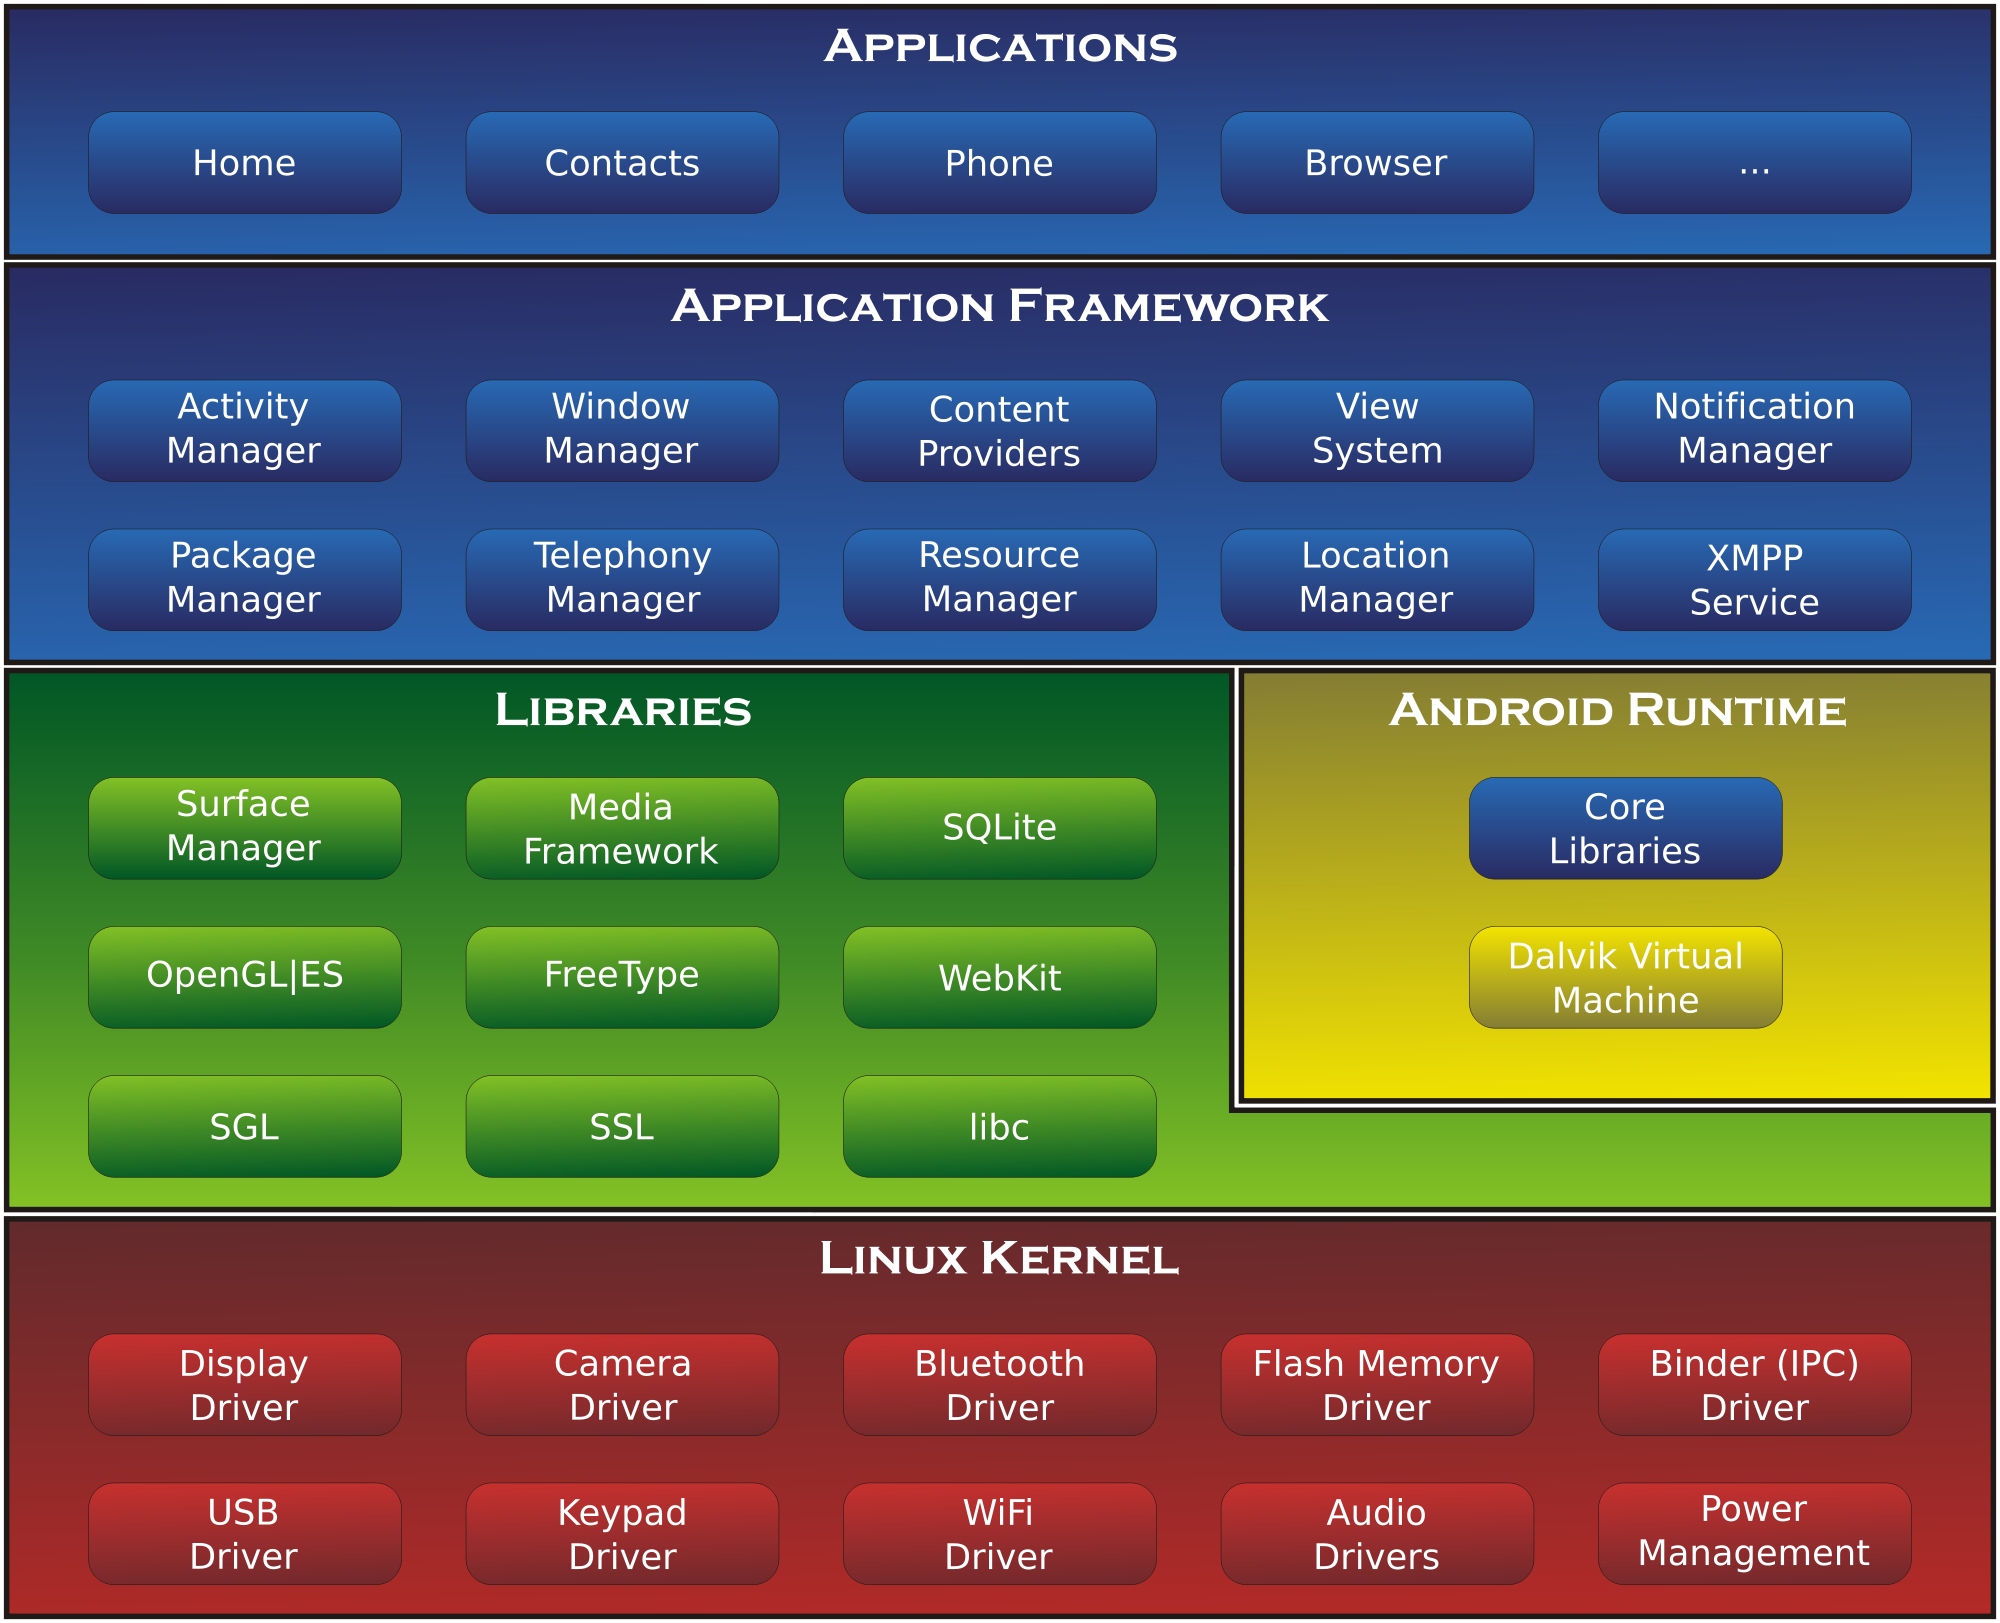
\includegraphics[width=0.9\textwidth]{AndroidSystemArchitecture.png}
	\bicaption[fig:androidSystemArchitecture]{这里将出现在插图索引中}{Android系统架构}{Fig}{Android system architecture}
\end{figure}

Android系统底层基于Linux内核,使用Linux内核文件形式的硬件驱动。Android系统中间层提供了常用的工具类库,包括轻量级数据库SQLite、浏览器引擎WebKit、图形程序接口OpenGL ES等,Android系统中间层还有Android Runtime,使用Dalvik虚拟机运行编译成字节码的程序。Android系统上层提供了窗口管理器、包管理器、资源管理器等能够让Android应用程序直接调用的工具和类库。

Android应用建立在Android系统三层架构之上,开发者通过调用Android系统提供的接口实现各种Android应用程序。图\ref{fig:androidSystemArchitecture}展现了整个Android系统的架构。

\subsection{Android应用模型}

一台Andorid设备里的每个Android应用拥有独立的UID(User Identifier),每个App都相当于Linux中独立用户,通过复用Linux的用户级隔离机制来实现Android应用的权限控制和数据隔离。

Android应用是组件化的,每个App包括运行在前台和后台的若干组件。每个组件可以当做单独的Linux进程,也可以多个组件共享一个Linux进程。同一个开发团队的不同App可以共享后台组件。

Android App的组件可以注册侦听某些事件,例如网络断开、屏幕开启、电池电量不足等,当事件发生时执行一段程序。一个组件在运行时也可以产生自定义事件,并可以指定把事件告知某个或者某一类组件。

\section{反馈信息}
\label{sec:replyInfo}

Android App使用过程中会产生许多数据,其中有些数据对于开发运营团队有价值,可以帮助完善优化程序,调整运营策略,提高用户体验。

Appetizer客户端SDK会收集用户会话信息、应用崩溃信息、ANR信息和黑白屏时长信息,本节的每个小节分别介绍了各个反馈信息的具体内容,对用户体验的影响及其数据价值。

\subsection{用户会话}

Android应用程序的用户会话,可以类比网站统计中的会话,简称session,这里可以称为App session,指的是用户使用一次App的整个过程,包括起止时间,打开的内容,内容跳转的路径,每个内容浏览的时间。

在Appetizer中,“页面”定义为Android中的Activity对象跟Fragment对象,是App session中用户浏览路径的基本单元。
对于一次App session的具体定义如下:

\begin{itemize}
	\item 从启动应用到关闭应用
	\item 从启动应用到应用退至后台,且在后台运行时间超过30秒
	\item 从启动应用到应用停留在某个页面未跳转时间超过30秒
\end{itemize}

例如用户在一次使用App的过程中跳转了多次页面,一个App session会包括多个浏览路径的信息。用户在将App切换至后台运行,超过30秒后再打开,Appetizer认为这是两次不同的会话,相当于用户打开了两次App。

用户会话可以用于统计日活跃用户,周活跃用户等数据,结合设备信息可以分析出日新增用户,老用户回流等更深层次的数据,这些分析数据在网站统计中已经较为成熟。除此之外,根据App session的浏览路径信息,可以分析出用户主要关注的内容,指导开发团队调整界面和内容,提高用户体验。

\subsection{Android应用崩溃}

Android应用程序最终以字节码的形式打包,所以通常使用能够运行在Java虚拟机上的程序语言进行开发,绝大部分Android应用使用Java语言开发,少部分使用Scala和Kotlin等JVM系语言开发,还有很少一部分使用Go语言和Swift语言开发。Android系统同时提供Native Development Kit,支持C/C++语言开发。

Android应用的崩溃可能发生在Dalvik层,以Java抛出未被捕获的异常(Exception)或者错误(Error)的形式发生,崩溃也可能发生在Native层,本篇文章和Appetizer只考虑收集App发生在Dalvik层的崩溃信息。

Android应用崩溃会影响用户的正常使用,崩溃的原因可能是程序逻辑代码本身的问题,设备碎片化导致的极少数设备运行问题,或者Android系统本身的问题。App崩溃会影响用户体验,在关键位置崩溃会导致App根本无法使用,崩溃会直接影响到用户量,对于用户量非常大的Android应用,低概率发生的崩溃就可能影响到成百上千万的用户。

Andorid应用崩溃信息收集功能可以及时把用户使用产生的崩溃问题告知开发团队,开发团队根据函数调用栈、设备型号、系统状态等信息对崩溃原因进行分析,及时解决问题,减少程序崩溃带来的负面影响。

\subsection{ANR}

Android ANR全称Application not responding,是指App运行某一段代码逻辑的时间过长,而无法响应用户的操作,通俗的说法就是程序卡死。

 在Android里,应用程序的响应性是由Activity Manager和WindowManager系统服务监视的,当它监测到以下情况中的一个时,系统就会针对特定的应用程序显示ANR:
 
 \begin{itemize}
 	\item 在5秒内没有响应用户的输入事件
 	\item BroadcastReceiver在10秒内没有执行完毕
 \end{itemize}

Android App和用户交互的界面由主线程更新,因此主线程又称为UI线程。应用程序长时间不响应用户输入的原因,可能是UI线程在长时间执行其他任务,例如数据库操作、网络操作、复杂的计算操作,也可能是UI线程死循环或者死锁。

间歇性发生ANR会让用户感觉应用卡顿,使用体验下降,长时间发生ANR会导致用户无法与应用交互,也就无法使用App,只能让系统强制关闭该应用。收集ANR发生时的函数调用栈信息和设备实时状态,发送给开发团队,有利于开发团队解决ANR问题,提升App的用户体验。

% TODO ANR截图

\subsection{启动黑白屏}

Android应用在启动的时候需要加载作为入口的Activity页面。在应用启动成功之后,入口Activity的布局内容加载完成之前,显示在设备屏幕上的是Android应用的主题背景,默认的通常是黑色或者白色,在这段时间用户只能看到黑色或白色的屏幕,称为Android应用启动时的黑白屏问题。

黑白屏问题是程序启动加载需要时间导致的必然存在的问题,无法彻底解决。黑白屏持续的时间和应用程序本身、Android系统版本、硬件性能、设备实时状态都有关,一些Android应用选择透明背景或者一张图片掩盖黑白屏问题,缓解用户在这段应用启动等待时间的急躁心理,应用启动后的等待时间过长会影响用户体验。

Appetizer客户端SDK能够记录每次Android应用启动后,加载入口Activity布局文件的等待时间,也就是黑白屏时间。该数据发送给开发团队,可以让开发团队判断启动加载时间长度是否能够接受,决定是否需要对程序进行权衡和优化,以减少应用启动后的等待时间,提升App的用户体验。

\section{本章小结}

本章介绍了Appetizer项目和所解决的问题相关的技术背景,为后文的设计和实现做铺垫。

\ref{sec:androidModel}节介绍了Android系统相关的背景知识,包括Android系统架构和Android应用组件化的模型。\ref{sec:replyInfo}节介绍了Appetizer客户端SDK所收集信息的相关背景知识,以及这些信息对开发团队的价值。
